\documentclass{scrreprt}
\usepackage{listings}
\usepackage{underscore}
\usepackage{graphicx}
\usepackage[bookmarks=true]{hyperref}
\usepackage[utf8]{inputenc}
\usepackage[english]{babel}
\usepackage{longtable}
\usepackage{float}
\usepackage{pdflscape}
\usepackage{array}
\usepackage{tabularray}

\UseTblrLibrary{booktabs}
\DefTblrTemplate{firsthead,middlehead,lasthead}{default}{}

\DefTblrTemplate{firstfoot}{default}{
  \UseTblrTemplate{caption}{default}
}

\DefTblrTemplate{middlefoot}{default}{
  \UseTblrTemplate{capcont}{default}
}

\DefTblrTemplate{lastfoot}{default}{
  \UseTblrTemplate{caption}{default}
}

\usepackage[
    a4paper,
    left=3cm,
    right=3cm,
    top=3cm,
    bottom=3cm
]{geometry}

\hypersetup{
    bookmarks=false,    % show bookmarks bar?
    pdftitle={Software Requirement Specification},    % title
    pdfauthor={Vo An Khoi},                     % author
    pdfsubject={SRS for Community Social Network LKForum},
    pdfkeywords={Website, SRS, Social Media},
    colorlinks=true,       % false: boxed links; true: colored links
    linkcolor=blue,       % color of internal links
    citecolor=black,       % color of links to bibliography
    filecolor=black,        % color of file links
    urlcolor=purple,        % color of external links
    linktoc=page            % only page is linked
}%
\def\myversion{1.0 }
\date{}
%\title{%

%}
\usepackage{hyperref}
\begin{document}

\begin{flushright}
    \rule{16cm}{5pt}\vskip1cm
    \begin{bfseries}
        \Huge{BUSINESS\\ REQUIREMENTS}\\
        \vspace{1.5cm}
        for\\
        \vspace{1.5cm}
        LKFORUM WEBSITE\\
        \vspace{1.5cm}
        \LARGE{Version \myversion}\\
        \vspace{1.5cm}
        Prepared by : Quach Gia Kiet\\
        Vo An Khoi\\
        \vspace{1.5cm}
        Submitted to : Nguyen Trinh Đong \\Lecturer\\
        \vspace{1.5cm}
        \today\\
    \end{bfseries}
\end{flushright}

\tableofcontents

\chapter{Objective and Scope}

\section{Project Objective}
The primary objective of the LKForum project is to design and build a modern, scalable, and highly interactive community platform. Unlike general social networks, LKForum focuses on autonomous community management, allowing users to create, configure, and moderate their own niche sub-forums (Communities).

The development focuses on delivering a high-quality system that ensures:
\begin{itemize}
    \item High performance for real-time interactions, including Instant Messaging and Notifications.
    \item Superior scalability to handle a large and growing number of concurrent communities and users.
    \item Robust moderation capabilities, integrating both automated (AI-assisted) and manual review processes.
    \item High standards for security and data privacy to protect user information and platform integrity.
\end{itemize}

\section{Project Scope}

The project scope includes the following modules:

\begin{itemize}
    \item \textbf{Identity \& Access Management:} Multi-factor authentication, SSO, and granular role-based access control.
    \item \textbf{Community Management:} Creation, configuration (public/private/18+), rule-setting, and membership handling.
    \item \textbf{Content Management:} Multi-format posts (text, image, video, poll), nested comments, and draft management.
    \item \textbf{Engagement System:} Real-time voting (upvote/downvote), saved posts, and activity history.
    \item \textbf{Communication Suite:} Real-time 1-1 messaging via WebSockets and an instant notification system.
    \item \textbf{Moderation \& Governance:} Report handling, user banning/muting, and content approval workflows.
    \item \textbf{Administration Dashboard:} Global system oversight, analytics, and platform-wide moderation.
\end{itemize}

\chapter{Business Requirements}

\section{Application Overview}

LKForum is a community-driven social network structured around ``Communities'' (sub-forums).

\begin{itemize}
    \item \textbf{Users} can discover and join communities based on interests.
    \item \textbf{Content} is categorized by communities, ensuring relevant discussions.
    \item \textbf{Decentralized Moderation:} Each community has its own set of rules and a dedicated moderation team (Owners/Moderators), reducing the burden on global administrators.
    \item \textbf{Real-time Experience:} The platform provides instant feedback, live messaging, and notifications.
\end{itemize}

\section{Domain Model}

\subsection{Domain Diagram (Conceptual)}

\begin{figure}[H]
    \centering
    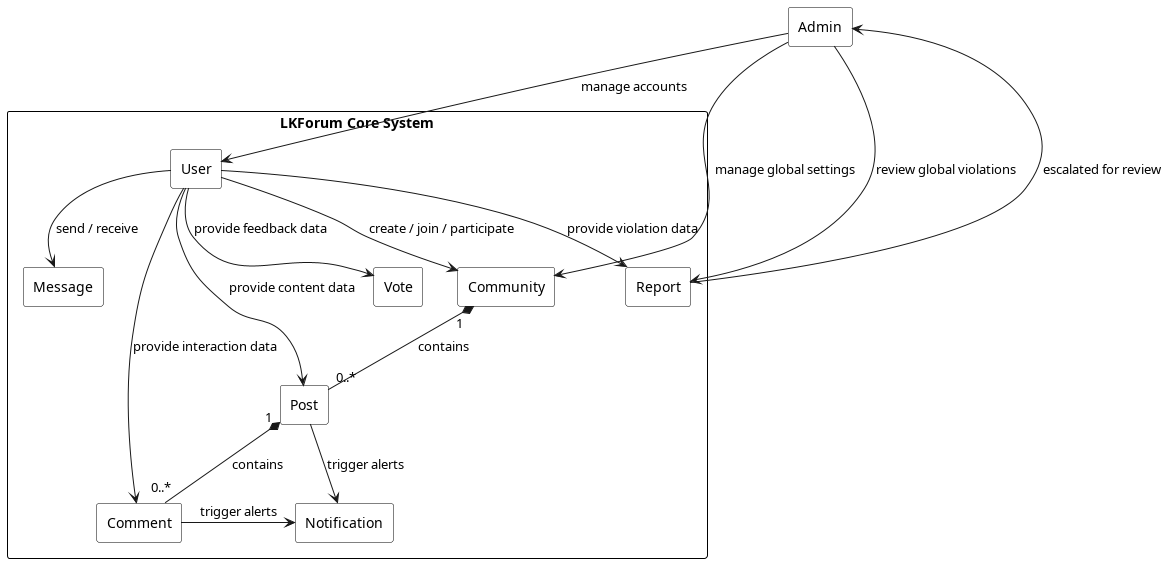
\includegraphics[width=0.9\textwidth]{diagrams/domain_model.png}
    \caption{Domain Model Diagram}
\end{figure}

\subsection{Domain Objects Description}

\begin{table}[H]
\centering

\begin{tblr}{
    width=\textwidth,
    hlines,
    vlines,
    row{1} = {font=\bfseries},
    rows = {valign=m},
    columns = {halign=c},
    colspec = {Q[c,1cm] Q[l,4cm] Q[l,8cm]}
}
\# & Object Name & Object Description \\

1 & User &
A registered identity with a profile, karma points, and activity history. \\

2 & Community &
A niche hub with specific topics, rules, and privacy settings. \\

3 & Post &
Content shared within a community (Text, Image, Video, or Poll). \\

4 & Comment &
A response to a post, supporting nested/threaded replies. \\

5 & Vote &
An expression of approval (Upvote) or disapproval (Downvote) on content. \\

6 & Message &
Direct communication content between users in a 1-1 chat. \\

7 & Notification &
Real-time alerts for replies, mentions, votes, or system messages. \\

8 & Report &
A user-generated complaint about content or behavior violating rules. \\
\end{tblr}

\caption{Domain Objects Description}

\end{table}

\section{Workflow}

\subsection{Content Lifecycle \& Moderation Workflow}

\begin{enumerate}
    \item \textbf{Creation:} A user creates a post in a community.
    \item \textbf{AI Screening:} The system automatically checks content for prohibited keywords/media.
    \item \textbf{Approval (Optional):} If the community requires post approval, the post is held in a \textit{Pending} state.
    \item \textbf{Moderation:} A Moderator/Owner reviews the post (Approve or Reject).
    \item \textbf{Publication:} Once approved, the post becomes public and triggers notifications to members.
\end{enumerate}

\subsection{Community Management Workflow}

\begin{enumerate}
    \item \textbf{Setup:} A user creates a community and becomes the Owner.
    \item \textbf{Configuration:} The Owner sets rules, privacy settings, and invites Moderators.
    \item \textbf{Governance:} Owners and Moderators monitor reports and can ban/mute users or remove content.
\end{enumerate}

\section{Use Cases and Actors}

\subsection{Use Case Diagram}

\begin{figure}[H]
    \centering
    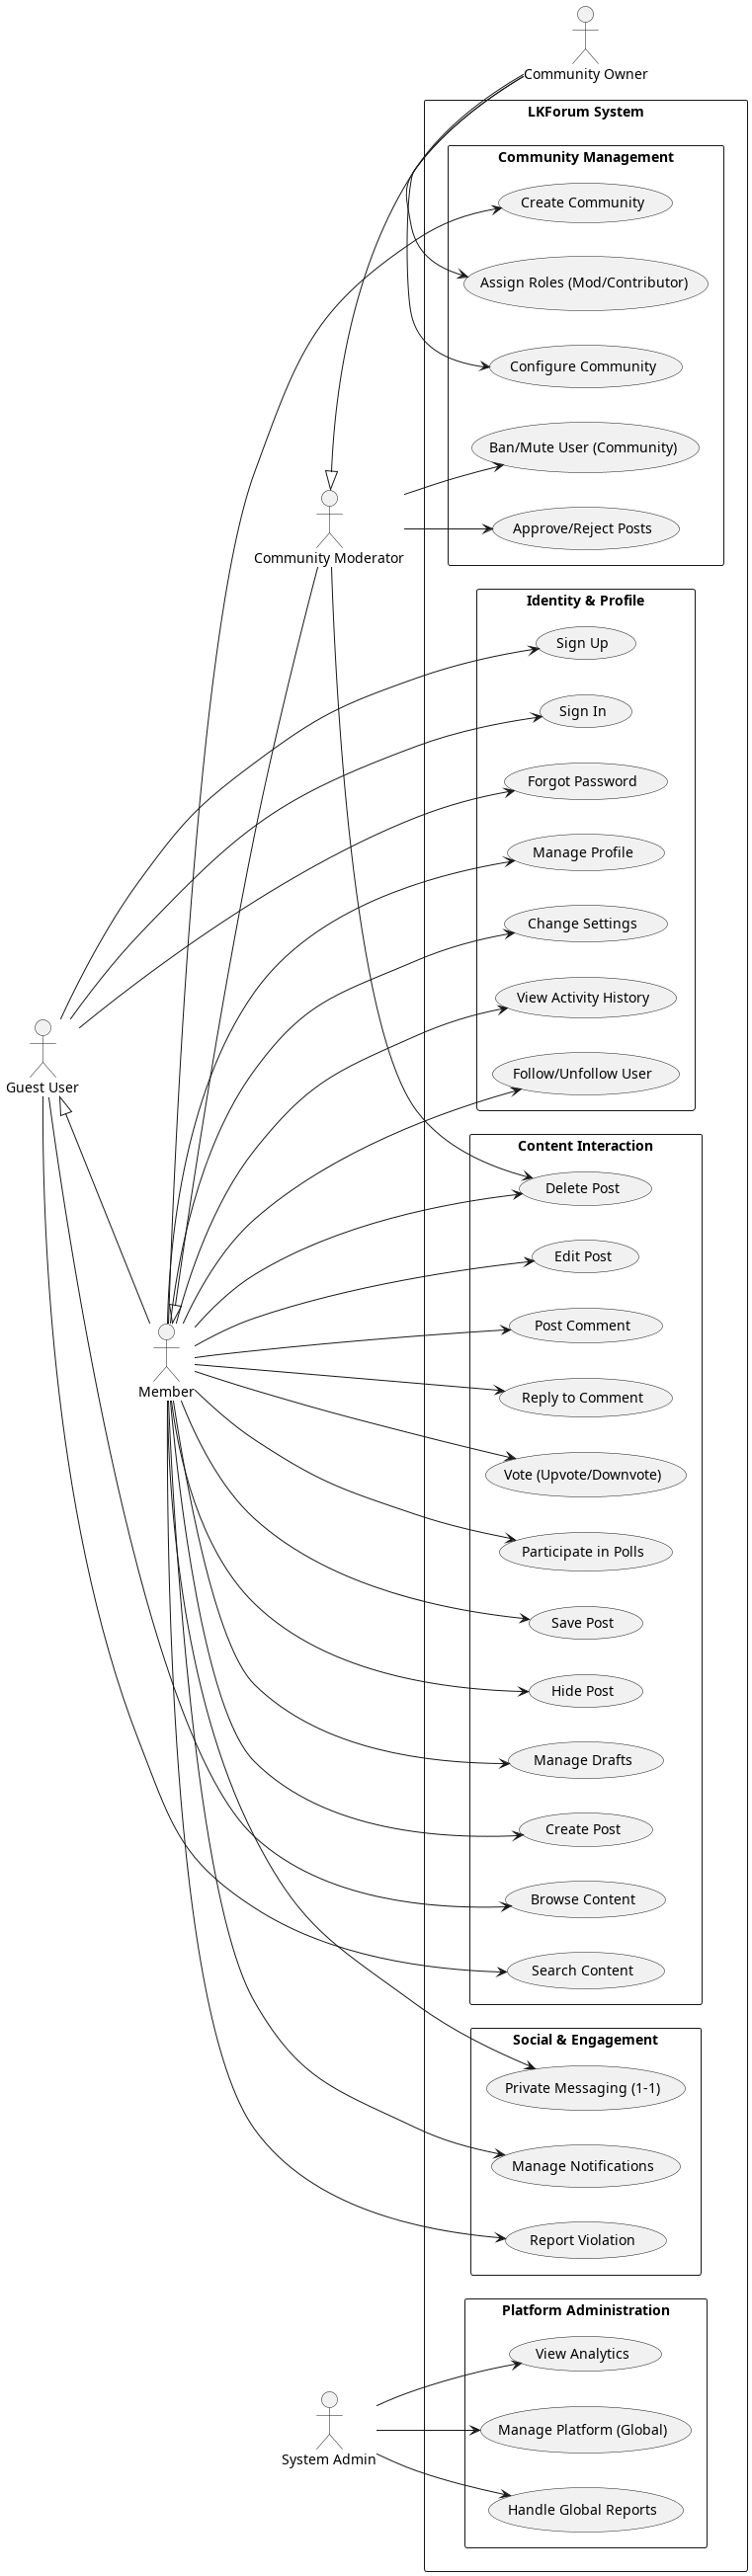
\includegraphics[
        width=\textwidth,
        height=0.85\textheight,
        keepaspectratio
    ]{diagrams/use_case_diagram.png}
    \caption{Use Case Diagram}
\end{figure}

\subsection{Description of Actors}

\begin{table}[H]
\centering
\label{tab:actors}
\begin{tblr}{
    width=\textwidth,
    hlines,
    vlines,
    row{1} = {font=\bfseries},
    rows = {valign=m},
    columns = {halign=c},
    colspec = {Q[c,1cm] Q[l,4cm] Q[l,8cm]}
}
ID & Actor Name & Definition \\

U-1 & Guest User &
Unauthenticated user; can browse public content and search. \\

U-2 & Member &
Authenticated user; can post, comment, vote, and message. \\

U-3 & Community Moderator &
Member with management rights in a specific community. \\

U-4 & Community Owner &
Creator of a community; can appoint moderators and change settings. \\

U-5 & System Admin &
Global administrator responsible for platform-wide health and safety. \\
\end{tblr}
\caption{Description of Actors}
\end{table}

\subsection{Description of Use Cases}

\noindent
\begin{longtblr}[
    caption = {Description of Use Cases},
    label = {tab:usecases}
]{
    width=\textwidth,
    hlines,
    vlines,
    row{1} = {font=\bfseries},
    rows = {valign=m},
    columns = {halign=c},
    colspec = {Q[c,1.2cm] Q[l,4.2cm] Q[l,7.2cm]}
}
\textbf{ID} & \textbf{Use Case Name} & \textbf{Definition} \\

UC-01 & \textbf{Sign Up} & Users create a new account by providing email, username, and password, verified via OTP. \\
UC-02 & \textbf{Sign In} & Authenticated access using credentials or linked Google OAuth account. \\
UC-03 & \textbf{Forgot Password} & Users reset their password through email verification (OTP). \\
UC-04 & \textbf{Manage Profile} & Users update personal information, including bio, avatar, and cover image. \\
UC-05 & \textbf{Change Settings} & Users configure account preferences (privacy, notifications, theme). \\
UC-06 & \textbf{View Activity History} & Users review their past posts, comments, and interactions. \\
UC-07 & \textbf{Follow/Unfollow User} & Users subscribe to another user's activity feed. \\
UC-08 & \textbf{Browse Content} & Users explore communities and view public posts without necessarily logging in. \\
UC-09 & \textbf{Search Content} & Users search for specific keywords, posts, users, or communities. \\
UC-10 & \textbf{Create Post} & Members publish new content (Text, Image, Video) within a selected community. \\
UC-11 & \textbf{Edit Post} & Members modify the content of their existing posts (stores edit history). \\
UC-12 & \textbf{Delete Post} & Members or Moderators remove posts from public view (soft delete). \\
UC-13 & \textbf{Post Comment} & Users add a response directly to a post. \\
UC-14 & \textbf{Reply to Comment} & Users respond to an existing comment (supporting nested threads). \\
UC-15 & \textbf{Vote on Content} & Users express approval (Upvote) or disapproval (Downvote) on posts/comments. \\
UC-16 & \textbf{Participate in Poll} & Users cast votes in community-created polls. \\
UC-17 & \textbf{Save Post} & Users bookmark posts for quick access later. \\
UC-18 & \textbf{Hide Post} & Users hide specific posts from their personal feed. \\
UC-19 & \textbf{Manage Drafts} & Users save unfinished posts as drafts and resume editing later. \\
UC-20 & \textbf{Private Messaging} & Users send and receive instant 1-1 messages via WebSocket. \\
UC-21 & \textbf{Manage Notifications} & Users view and clear real-time alerts for engagement and system updates. \\
UC-22 & \textbf{Report Violation} & Users flag inappropriate content or behavior for moderator review. \\
UC-23 & \textbf{Create Community} & Users establish a new niche forum and become the ``Owner.'' \\
UC-24 & \textbf{Approve/Reject Post} & Moderators review pending posts before they appear in the community. \\
UC-25 & \textbf{Ban/Mute User} & Moderators restrict a user's ability to participate within a community. \\
UC-26 & \textbf{Configure Community} & Owners adjust rules, privacy settings, and appearance of their community. \\
UC-27 & \textbf{Assign Roles} & Owners appoint other members as Moderators or Contributors. \\
UC-28 & \textbf{Handle Global Reports} & System Admins review and act on platform-wide violation reports. \\
UC-29 & \textbf{Manage Platform} & System Admins ban/unban users or communities globally. \\
UC-30 & \textbf{View Analytics} & System Admins monitor platform statistics (DAU, growth, content volume). \\
\end{longtblr}

\section{Security Matrix}

\noindent
\begin{longtblr}[
    caption = {Security Matrix}
]{
    width=\textwidth,
    hlines,
    vlines,
    row{1} = {font=\bfseries},
    rows = {valign=m},
    columns = {halign=c},
    colspec = {Q[c,0.8cm] Q[l,5cm] Q[c,1cm] Q[c,1.5cm] Q[c,1cm] Q[c,1.2cm] Q[c,1.2cm]}
}
\# & Function & Guest & Member & Mod & Owner & Admin \\

1 & Sign Up / Sign In / Forgot Password & X & X & X & X & X \\
2 & Manage Profile \& Settings &  & X & X & X & X \\
3 & Follow / Unfollow User &  & X & X & X & X \\
4 & Browse Public Content \& Search & X & X & X & X & X \\
5 & View Own Activity History &  & X & X & X & X \\
6 & Create Post / Comment / Reply &  & X & X & X & X \\
7 & Edit / Delete Own Content &  & X & X & X & X \\
8 & Vote / Participate in Polls &  & X & X & X & X \\
9 & Save / Hide Post / Manage Drafts &  & X & X & X & X \\
10 & Send/Receive Private Messages &  & X & X & X & X \\
11 & Receive Notifications &  & X & X & X & X \\
12 & Report Violations &  & X & X & X & X \\
13 & Create New Community &  & X & X & X & X \\
14 & Approve / Reject / Pin Posts &  &  & X & X & X \\
15 & Delete Any Post (In Community) &  &  & X & X & X \\
16 & Ban / Mute User (In Community) &  &  & X & X & X \\
17 & Configure Community Settings &  &  &  & X & X \\
18 & Assign Roles (Mod/Contributor) &  &  &  & X & X \\
19 & Handle Global Reports &  &  &  &  & X \\
20 & Global User / Community Ban &  &  &  &  & X \\
21 & View System Analytics &  &  &  &  & X \\
\end{longtblr}

\section{User Story}

\subsection{Guest Users}

\begin{longtblr}[
    caption = {Guest User Stories},
    label = {tab:guest_user_stories}
]{
    width=\textwidth,
    hlines,
    vlines,
    row{1} = {font=\bfseries},
    rows = {valign=m},
    colspec = {Q[c,1.2cm] Q[l,12cm]},
    row{1} = {font=\bfseries, halign=c},
}
\textbf{ID} & \textbf{User Story} \\

US-01 & As a Guest User, I want to browse posts so that I can explore content without creating an account. \\
US-02 & As a Guest User, I want to view posts and comments so that I can read discussions. \\
US-03 & As a Guest User, I want to search for keywords so that I can find relevant content. \\
US-04 & As a Guest User, I want to search for communities so that I can discover topics of interest. \\
US-05 & As a Guest User, I want to view user profiles so that I can learn about content creators. \\
US-06 & As a Guest User, I want to be prompted to sign up when attempting restricted actions so that I understand the benefits of creating an account. \\
US-07 & As a Guest User, I want to sign up with my email and verify via OTP so that I can securely create an account. \\
\end{longtblr}

\subsection{Members}

\begin{longtblr}[
    caption = {Member User Stories},
    label = {tab:member_user_stories}
]{
    width=\textwidth,
    hlines,
    vlines,
    row{1} = {font=\bfseries},
    rows = {valign=m},
    colspec = {Q[c,1.2cm] Q[l,12cm]},
    row{1} = {font=\bfseries, halign=c},
}
\textbf{ID} & \textbf{User Story} \\

US-08 & As a Member, I want to sign in using my Google account so that I can quickly access the platform without creating a new password. \\
US-09 & As a Member, I want to sign in using my email and password so that I can access my account securely. \\
US-10 & As a Member, I want to customize my profile with a bio so that I can describe myself. \\
US-11 & As a Member, I want to upload an avatar so that other users can recognize me. \\
US-12 & As a Member, I want to upload a profile banner so that I can personalize my profile page. \\
US-13 & As a Member, I want to create a text post so that I can share content with others. \\
US-14 & As a Member, I want to upload images to my post so that I can share visual content. \\
US-15 & As a Member, I want to create a poll in my post so that I can gather opinions from others. \\
US-16 & As a Member, I want to save my post as a draft so that I can edit and publish it later. \\
US-17 & As a Member, I want to upvote posts so that valuable content is highlighted. \\
US-18 & As a Member, I want to downvote posts so that low-quality content is less visible. \\
US-19 & As a Member, I want to upvote comments so that helpful responses are recognized. \\
US-20 & As a Member, I want to downvote comments so that unhelpful responses are less visible. \\
US-21 & As a Member, I want to create, modify, and delete comments under a post. \\
US-22 & As a Member, I want to reply to a specific comment so that conversations remain structured. \\
US-23 & As a Member, I want to receive notifications when someone replies to my post or comment so that I stay updated. \\
US-24 & As a Member, I want to receive notifications when someone mentions me so that I can respond quickly. \\
US-25 & As a Member, I want to follow other users so that I can see their activities in my feed. \\
US-26 & As a Member, I want to view posts from users I follow so that I can stay updated with their content. \\
US-27 & As a Member, I want to send private messages to other users so that I can communicate one-on-one. \\
US-28 & As a Member, I want to report inappropriate content so that I can help maintain a safe community. \\
\end{longtblr}

\subsection{Community Owners \& Moderators}

\begin{longtblr}[
    caption = {Community Owner and Moderator User Stories},
    label = {tab:community_user_stories}
]{
    width=\textwidth,
    hlines,
    vlines,
    row{1} = {font=\bfseries},
    rows = {valign=m},
    colspec = {Q[c,1.2cm] Q[l,12cm]},
    row{1} = {font=\bfseries, halign=c},
}
\textbf{ID} & \textbf{User Story} \\

US-29 & As a Community Owner, I want to create a community so that I can build a space for specific topics. \\
US-30 & As a Community Owner, I want to define community rules so that members understand acceptable behavior. \\
US-31 & As a Community Owner, I want to set privacy settings (public or private) so that I can control access to the community. \\
US-32 & As a Community Owner, I want to assign moderator roles to members so that they can help manage the community. \\
US-33 & As a Community Moderator, I want to review and approve pending posts so that only appropriate content is published. \\
US-34 & As a Community Moderator, I want to remove posts or comments so that I can enforce community rules. \\
US-35 & As a Community Moderator, I want to mute users so that they temporarily cannot interact. \\
US-36 & As a Community Moderator, I want to ban users so that I can prevent disruptive behavior. \\
\end{longtblr}

\subsection{System Administrators}

\begin{longtblr}[
    caption = {System Administrator User Stories},
    label = {tab:admin_user_stories}
]{
    width=\textwidth,
    hlines,
    vlines,
    row{1} = {font=\bfseries},
    rows = {valign=m},
    colspec = {Q[c,1.2cm] Q[l,12cm]},
    row{1} = {font=\bfseries, halign=c},
}
\textbf{ID} & \textbf{User Story} \\

US-37 & As a System Admin, I want to view a dashboard with system analytics so that I can monitor platform performance. \\
US-38 & As a System Admin, I want to review reports escalated from communities so that I can take appropriate action. \\
US-39 & As a System Admin, I want to ban users globally so that malicious users are removed from the platform. \\
US-40 & As a System Admin, I want to remove or restrict communities so that harmful communities are controlled. \\
\end{longtblr}

\chapter{Appendix}

\section{Glossary}

\begin{itemize}
    \item \textbf{Karma:} A reputation score based on the net value of upvotes and downvotes received.
    
    \item \textbf{Sub-forum:} Synonymous with ``Community'' in LKForum.
    
    \item \textbf{SSO:} Single Sign-On (Google Authentication).
    
    \item \textbf{OTP:} One-Time Password sent via email for verification.
\end{itemize}

\section{Open Issues}

\begin{itemize}
    \item Implementation of cross-posting (sharing posts across multiple communities).
    
    \item Automated AI moderation for image/video content (currently focusing on text).
    
    \item Integration of a global search engine (Elasticsearch).
\end{itemize}

\end{document}
